\section{Theorie}
\label{sec:Theorie}

In der Werkstofftechnik stellt der Elastizitätsmodul $E$ einen wichtigen Materialkennwert dar.
Der Elastizitätsmodul ist ein Faktor, welcher die Gestaltsdeformation eines Körpers unter Wirkung einer Normalspannung oder eines Druckes $\sigma$ beschreibt.

Allgemein werden Kräfte, welche an der Oberfläche eines Körpers angreifen, als Spannung bezeichnet. \\
Als Schub- oder Tangentialspannung wird hierbei die oberflächenparallele Komponente, als \textbf{Normalspannung} $\sigma$ die zur Oberfläche senkrechte Komponente der Spannung, bezeichnet.\\
Ist die, durch die Normalspannung verursachte, relative Änderung einer linearen Körperdimension (zum Beispiel einer Länge $L$) hinreichend klein,
besteht ein linearer Zusammenhang zwischen der angreifenden Spannung $\sigma$ und der relativen Änderung $\frac{\Delta L}{L}$ mit dem Elastizitätsmodul $E$ als Proportionalitätsfaktor.
\begin{equation}
	\label{eqn:hook}
	\sigma=E \cdot \frac{\Delta L}{L} \mathrm{.}
\end{equation}
Dieser Zusammenhang wird als \textbf{Hooksches Gesetz} bezeichnet.\\
Falls die Längenänderung $\Delta L$ direkt genau bestimmt werden kann, könnte prinzipiell nach Formel \eqref{eqn:hook} der Elastizitätsmodul bestimmt werden.
Dafür sind allerdings hochpräzise Messgeräte notwendig. Daher wird in diesem Versuch der Elastizitätsmodul über die Biegung eines Probestabes -- bedingt durch eine angreifende Kraft -- untersucht.\\
Die Durchbiegung $D(x)$ ist bei ansonsten unveränderten Eigenschaften des Probestabes relativ groß gegenüber $\Delta L$ und lässt daher auch bei weniger präzisen Messgeräten eine Bestimmung des Elastizitätsmoduls $E$ zu.

\subsection{Berechnung der Durchbiegung eines homogenen Stabes}

Greift am Stabende eine Kraft $F$ an, so verursacht diese auf jedem Querschnitt $Q$ des Probestabes ein Drehmoment $M_{\mathrm{F}}$, sodass der Stab aus seiner Ruhelage ausgelenkt wird. Das Drehmoment $M_{\mathrm{F}}$ ergibt sich hierbei aus dem Produkt zwischen dem Hebelarm für den betrachteten Querschnitt $Q$ des Stabes und angreifender Kraft $F$.
\\Aufgrund dieser Durchbiegung der Probe treten in dieser Normalspannungen auf, die der Deformation entgegenwirken.
In den oberen Schichten des Stabes treten Zugspannungen auf, in den unteren Schichten entsprechend Druckspannungen.
\\Mittig des Stabes (in Abbildung \ref{fig:Durchbiegung} durch eine gestrichelte Linie dargestellt) liegt die sogenannte \textbf{neutrale Faser}. In dieser treten keine Spannungen auf.
\begin{figure}
	\centering
	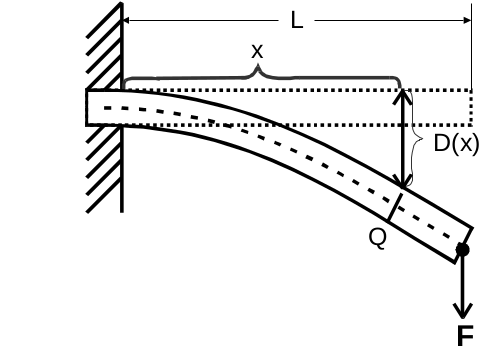
\includegraphics[width=0.7\textwidth]{Bilder/durchbiegungstab.png}
	\caption{Durchbiegung des einseitig eingespannten Stabes bei angreifender Kraft $F$ am anderen Stabende. \cite{Anleitung}}
	\label{fig:Durchbiegung}
\end{figure}
Da die Zug- und Druckspannung an jedem Querschnitt $Q$ des Probestabes entgegengesetzt gleich sind, erzeugen sie ein Drehmoment $M_{\mathrm{\sigma}}$ auf $Q$.
Die Durchbiegung $D(x)$ erreicht einen stationären Zustand, wenn $M_{\mathrm{F}}$ und $M_{\mathrm{\sigma}}$ übereinstimmen. \\
Da $M_{\mathrm{\sigma}}$ das Integral des Produkts aus $y$ und $\sigma(y)$ über den Querschnitt $Q$ des Stabes ist, ergibt sich

\begin{equation}
	\label{eqn:momentengleichung}
	M_{\mathrm{F}}=M_{\mathrm{\sigma}} \Rightarrow F(L-x)=\int_{\symup{Q}}^{} y \cdot \sigma(y) \symup{dq} \mathrm{.}
\end{equation}
Das $\symup{dq}$ ist hierbei das Flächenelement mit Abstand $y$ von der neutralen Faser. \\
Die Normalspannung $\sigma(y)$ lässt sich durch das Hooksche Gesetz \eqref{eqn:hook} bestimmen.\\
Unter Verwendung (differential-) geometrischer Überlegungen lässt sich Gleichung \eqref{eqn:momentengleichung} schreiben als
\begin{equation}
	\label{eqn:integralmomentengleichung}
	F(L-x)=E \, \frac{\symup{d}^2}{\symup{d}x^2} \int_{\symup{Q}}^{} y^2 \symup{dq}=I \cdot E\, \frac{\symup{d}^2}{\symup{d}x^2} \mathrm{.}
\end{equation}
Analog zum Massenträgheitsmoment $\theta$ wird $I$ als \textbf{Flächenträgheitsmoment} definiert.
Die Integration von Gleichung  \eqref{eqn:integralmomentengleichung} liefert somit sofort einen Ausdruck für die Auslenkung $D$ in Abhängigkeit zu $x$

\begin{equation}
	\label{eqn:d_x_einseitig}
	D(x)=\frac{F}{2EI}\left(Lx^2-\frac{x^3}{3}\right) \text{.}
\end{equation}
Hierbei ist $L$ die Länge des Stabes vom eingespannten Ende bis zum Punkt, an dem die Kraft $F$ angreift und $x$ ist der Abstand zwischen dem Einspannpunkt und dem Messpunkt (vgl. Abbildung \ref{fig:Durchbiegung}).

Greift die Kraft $F$ bei beidseitiger Einspannung in der Mitte des Stabes an, wirkt nur noch die halbe Kraft an der Querschnittsfläche $Q$. Für die beiden Stabhälften wirken unterschiedliche Drehmomente $M_{\mathrm{F}}$ und für die Durchbiegung ergeben sich die beiden Gleichungen
\begin{equation}
	\label{eqn:d_x_beidseitig_eins}
	D(x)=\frac{F}{48EI}\left(3L^2x-4x^3\right) \mathrm{ für }\,\, 0\leq x\leq\frac{L}{2} \mathrm{,}
\end{equation}
\begin{equation}
	\label{eqn:d_x_beidseitig_zwei}
	D(x)=\frac{F}{48EI}\left(4x^3-12 Lx^2+9 L^2x-L^3\right) \mathrm{ für }\,\, \frac{L}{2}\leq x \leq L \mathrm{.}
\end{equation}
